\section{Specifications}
\newcounter{rulei}[subsection]
\newcommand{\rcnii}{\stepcounter{rulei}\arabic{section}.\arabic{subsection}.\arabic{rulei}}
\renewcommand{\labelenumi}{\rcnii}

\subsection{Arena}
\begin{enumerate}
\item The match arena floor is an $8m \times 8m$ square.
 The tolerance of the two arena dimensions is $\pm0.25m$.
\item The floor of the arena is made of white plastic coated hardboard.
 White Gaffer tape will be in place over the joints between hardboard sheets.
\item The arena walls are $600\pm30mm$ high and are made of the same material as the arena floor.
\item The arena is encased in a scaffolding structure, which is $1.4m \pm0.1m$ tall.	\textbf{@check}
\end{enumerate}

\subsection{The Tower}
\label{tower}
\begin {enumerate} 
\item The tower will be located in the centre of the arena and will be orientated in line with the arena sides.
\item The tower has a footprint of $2m \times 1m$.
\item Robots should not intentionally damage or destroy the tower.
\item The tower is painted green.
\end {enumerate}

\subsection{Tokens}
\label{tokens}
\begin {enumerate} 
\item Tokens will be cubes of side $45mm$, to an accuracy of $\pm5mm$.
 Each team's kit contains a small number of these.
\item Tokens will weigh between WEIGHT and WEIGHT.	\textbf{@check}
\item A token only accounts to a team's score when it is successfully collected by the robot.
\item Robots should not intentionally damage or destroy tokens.
\item The tokens will be painted red and blue, with each scoring as described in the Game Rules section.
\end {enumerate}

\subsection{Robot Flags}
\label{sec:flags}
All robots must have a flagpole so that two flags can be mounted upon it:
\begin{description}
\item[Team Flag] The team flag is to be designed and created by the team.
 The team flag allows the robot to be easily identified.
 This flag must be mounted between $700mm$ and $900mm$ off the ground.
 It must not extend more than $200mm$ from the flagpole.

The team flag must not sag below $700mm$ above the ground.
\item[Match Flag] The match flag is to be supplied by Student Robotics at the start of every match.
 The match flag will slot over the top $100mm$ of the flagpole.
 The top $100mm$ of the flagpole must have an external diameter of $5\pm1mm$ so that the match flag can slot over it.
 The match flags have an end-cap so that they will not slide down the flagpole.
\end{description}

The flagpole must be removable so that the robot can be placed within a box to check the size limit.
A diagram of the flagpole arrangement can be found in figure~\ref{fig:flag}.

\begin{figure}
\begin{center}
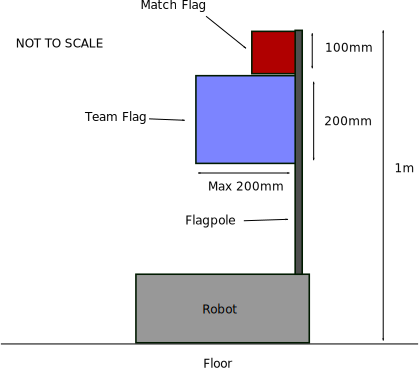
\includegraphics[keepaspectratio, scale =1]{./images/flag.png}
\caption{\label{fig:flag}Flagpole Dimensions}
\end{center}
\end{figure}
\clearpage
